\documentclass{article}

\usepackage[margin=1in]{geometry}     %for 1inch margins that play nice with fancyhdr
\usepackage{amsmath,amssymb}          % math and junk
\usepackage{fancyhdr}                 % for a nice running header and footer
\usepackage{lastpage}                 % for nice "X of Y" footer
\usepackage[per-mode=symbol]{siunitx} % for nice units and junk!
\usepackage{gnuplot-lua-tikz}         % enable tikz plots made from gnuplot
\usepackage{float}                    % [H] option for floats
\usepackage[american]{circuitikz}     % for teh circuit diagrams
\usepackage[hidelinks]{hyperref}                 % get those sweet, sweet, links
\usepackage{framed}                   % for framed titlepage

% unused, but common for other experiments
%\usepackage{rotating}                 % for sideways stuff!
%\usepackage{cancel}                   % for `canceling out' parts of equations. fancy!
%\usepackage{mdwlist}                  % itemize* and friends
%\usepackage{verbatim}                 % for \verbatiminput command and comment environment
%\usepackage[colorinlistoftodos]{todonotes}                % todo's, if used/needed
%\usepackage{multirow}                 % for multi-row spans in tabular environment


% values!
\newcommand{\docAuthor}{Sean Barag}
\newcommand{\docCoAuthor}{None}
\newcommand{\ta}{Kaloyan Popov}
\newcommand{\docTitle}{PSpice Computer Simulation of Electronic Circuits}
\newcommand{\courseName}{ECE-L303}
\newcommand{\labNum}{Lab 2}
\newcommand{\labSec}{062}
\newcommand{\dueDate}{8 October 2011}
\newcommand{\perfDate}{30 September 2011}

% paths
\graphicspath{{$HOME/texmf/graphics/}}


% meta-data
\pdfinfo{
	/Title    (\labNum: \docTitle)
	/Author   (\docAuthor)
	/Keywords (\docTitle, \labNum)
}

% for fancy header
\pagestyle{fancy}
\lhead{\courseName\ $|$ \labSec}
\chead{\labNum: \docTitle}
\rhead{\docAuthor}
\cfoot{\thepage\ of \pageref{LastPage}}

% title info
\title{\courseName\ \labNum: \\ \docTitle}
\author{\docAuthor}
\date{}

% shortcuts, cause I'm lazy
\newcommand{\bs}[1]{\boldsymbol{#1}}
\newcommand{\tbf}[1]{\textbf{#1}}

\begin{document}
% Cover page written by Bryndon Blackburn
% Originally written by Bryndon Blalckburn
\begin{titlepage}
	\begin{center}
		\includegraphics[scale = 0.50]{DrexelLogo.pdf}
	\end{center}

	\large
	\begin{framed}
		\begin{center}
			Electrical and Computer Engineering Dept. \\
			Electrical Engineering Laboratory III, ECE-L303 \\
		\end{center}
	\end{framed} \vspace{50pt}

	\begin{description}
		\item[Title:]\labNum: \docTitle
		\item[Author:] \docAuthor
		\item[Partner:] \docCoAuthor
		\item[Instructor:] \ta
		\item[Section:] \labSec
		\item[Date Performed:] \perfDate
		\item[Date Due:] \dueDate
		\item[Date Received:]
	\end{description}
\end{titlepage}


% Blank page so two-sided printing leaves the cover page on its own sheet
\thispagestyle{empty}
\newpage
\mbox{}

\maketitle
\setcounter{page}{1} % fixes page numbering issues caused by cover sheet
\tableofcontents % this helps
\pagebreak
\listoffigures   % there's over 9000 figures

\newpage % I want object to be at the top of a new page
\section{Object}
The purpose of experiment five was to provide useful experience with an analog
to digital converter (ADC), as well as to inform the student of the device's
behavior and applications.


\section{Circuit Diagrams}
\begin{figure}[H]
	\centering
	\begin{circuitikz}
	% body
	\draw[ultra thick] (-2, -4) rectangle (2, 4);

	% chip name
	\draw (0,0) node[rotate=90] {DAC0808};

	% -------------------- top --------------------
	\draw
	(0, 4) node[above left] {13} node[below] {$V_\text{CC}$}
		to [short, -o] ++(0, 1) node[above] {+\SI{5}{\volt}};


	% -------------------- left pins --------------------

	% resistors, LEDs, and pin ames
	\foreach \y in {7, ..., 0}
	{
		\draw (-2, \y-3.5) node[right] (b\y) {B\y}
		to [short, -o] ++(-0.5, 0);
	}

	% pin numbers
	\foreach \pin in {5,...,12}
	{
		\draw (-2, 8.5-\pin) node[above left] {\pin};
	}

	% LSB and MSB
	\draw (b7) node[right=4.5pt] {(MSB)}
	(b0) node[right=4.5pt] {(LSB)};

	% digital inputs label
	\path[draw, text centered ] (-3, 4) -- node[rectangle, fill=white, rotate=90] {Digital Inputs} (-3, -4);
	\draw
	(-3, 4)  -- ++(.5, 0)
	(-3, -4) -- ++(.5, 0);

	% -------------------- right pins --------------------

	% Vee and cap
	\draw
	(0, -4) node[below right] {3} node[above]{$V_\text{EE}$}
		to [short, -o] ++(0, -1.5) node[below] {\SI{-15}{\volt}}
	(2, -3.5) node[above right] {16} to [short] ++(1, 0) to [C, l=\SI{0.1}{\micro\farad}] ++(0, -1.5)
		to [short] ++(-3, 0);

	% pin 4
	\draw
	(2, -1) node[above right] {4} to [short] ++(1, 0)
		to [R, l=\SI{5}{\kilo\ohm}] ++(0, -1.5) node[ground] {}
	(3.5, -1) node[right] {$V_0$} to [short, i_=$I_0$, o-] ++(-.5, 0);

	% pins 15 & 2
	\draw
	(2, .5) node[above right] {2} to [short] ++(2.5, 0) node[ground] {}
		to [short] ++(0, 1)
	(2, 1.5) node[above right] {15} to [short] ++(.5, 0)
		to [R, l=\SI{5}{\kilo\ohm}] ++(2, 0);

	% pins 14
	\draw
	(2, 3.5) node[above right] {14} node[left] {$V_\text{REF}$} to [short] ++(.5, 0)
		to [R, l=\SI{5}{\kilo\ohm}, -o] ++(2, 0) node[below] {+\SI{5}{\volt}};


	% = - V_\text{REF} \left( \frac{A_1}{2} + \frac{A_2}{4} + \ldots + \frac{A_8}{256} \right)$}
\end{circuitikz}

	\parbox{.6\textwidth}{
	\caption[Digital-to-Analog IC schematic]{Circuit schematic provided in the
	lab instructions, describing the layout of the pre-built circuit used in
	experiment six.}
	\label{fig:dacSchem}}
\end{figure}


\section{Graphs \& Data}
\begin{table}[H]
	\centering
	\begin{tabular}{|c|c|c|}
	\hline
	$\boldsymbol{V_\mathrm{PS}}$ \tbf{(\si{\volt})} &
		$\boldsymbol{V_\mathrm{P-P}}$ \tbf{(\si{\volt})} &
			$\boldsymbol{f}$ \tbf{(\si{\kilo\hertz})} \\ \hline
	30		& 26.41		& 3.205 \\ \hline
	25		& 21.56		& 3.210 \\ \hline
	20		& 16.88		& 3.236 \\ \hline
	15		& 12.05		& 3.226 \\ \hline
	10		& 7.344		& 3.231 \\ \hline
	5		& 2.656		& 3.273 \\ \hline
\end{tabular}
\\
	\parbox{.6\textwidth}{
	\caption[Voltage Sweep Data]{Data recorded from the voltage sweep,
		measuring the peak-to-peak voltage~($V_\mathrm{P-P}$) and
		frequency~($f$) on an oscilloscope as a function of the power supply
		voltage~($V_\mathrm{PS}$).}
	\label{tab:vSweepData}}
\end{table}

\begin{figure}[H]
	\centering
	\begin{tikzpicture}[gnuplot]
%% generated with GNUPLOT 4.4p2 (Lua 5.1.4; terminal rev. 97, script rev. 96a)
%% Sat 15 Oct 2011 11:14:53 PM EDT
\gpsolidlines
\gpcolor{gp lt color axes}
\gpsetlinetype{gp lt axes}
\gpsetlinewidth{1.00}
\draw[gp path] (1.320,0.985)--(8.830,0.985);
\gpcolor{gp lt color border}
\gpsetlinetype{gp lt border}
\draw[gp path] (1.320,0.985)--(1.500,0.985);
\node[gp node right] at (1.136,0.985) { 0};
\gpcolor{gp lt color axes}
\gpsetlinetype{gp lt axes}
\draw[gp path] (1.320,1.529)--(8.830,1.529);
\gpcolor{gp lt color border}
\gpsetlinetype{gp lt border}
\draw[gp path] (1.320,1.529)--(1.500,1.529);
\node[gp node right] at (1.136,1.529) { 5};
\gpcolor{gp lt color axes}
\gpsetlinetype{gp lt axes}
\draw[gp path] (1.320,2.072)--(8.830,2.072);
\gpcolor{gp lt color border}
\gpsetlinetype{gp lt border}
\draw[gp path] (1.320,2.072)--(1.500,2.072);
\node[gp node right] at (1.136,2.072) { 10};
\gpcolor{gp lt color axes}
\gpsetlinetype{gp lt axes}
\draw[gp path] (1.320,2.616)--(1.504,2.616);
\draw[gp path] (3.892,2.616)--(8.830,2.616);
\gpcolor{gp lt color border}
\gpsetlinetype{gp lt border}
\draw[gp path] (1.320,2.616)--(1.500,2.616);
\node[gp node right] at (1.136,2.616) { 15};
\gpcolor{gp lt color axes}
\gpsetlinetype{gp lt axes}
\draw[gp path] (1.320,3.159)--(1.504,3.159);
\draw[gp path] (3.892,3.159)--(8.830,3.159);
\gpcolor{gp lt color border}
\gpsetlinetype{gp lt border}
\draw[gp path] (1.320,3.159)--(1.500,3.159);
\node[gp node right] at (1.136,3.159) { 20};
\gpcolor{gp lt color axes}
\gpsetlinetype{gp lt axes}
\draw[gp path] (1.320,3.703)--(8.830,3.703);
\gpcolor{gp lt color border}
\gpsetlinetype{gp lt border}
\draw[gp path] (1.320,3.703)--(1.500,3.703);
\node[gp node right] at (1.136,3.703) { 25};
\gpcolor{gp lt color axes}
\gpsetlinetype{gp lt axes}
\draw[gp path] (1.320,4.246)--(8.830,4.246);
\gpcolor{gp lt color border}
\gpsetlinetype{gp lt border}
\draw[gp path] (1.320,4.246)--(1.500,4.246);
\node[gp node right] at (1.136,4.246) { 30};
\gpcolor{gp lt color axes}
\gpsetlinetype{gp lt axes}
\draw[gp path] (1.320,4.790)--(8.830,4.790);
\gpcolor{gp lt color border}
\gpsetlinetype{gp lt border}
\draw[gp path] (1.320,4.790)--(1.500,4.790);
\node[gp node right] at (1.136,4.790) { 35};
\gpcolor{gp lt color axes}
\gpsetlinetype{gp lt axes}
\draw[gp path] (1.320,0.985)--(1.320,4.790);
\gpcolor{gp lt color border}
\gpsetlinetype{gp lt border}
\draw[gp path] (1.320,0.985)--(1.320,1.165);
\node[gp node center] at (1.320,0.677) { 0};
\gpcolor{gp lt color axes}
\gpsetlinetype{gp lt axes}
\draw[gp path] (2.572,0.985)--(2.572,2.425);
\draw[gp path] (2.572,3.349)--(2.572,4.790);
\gpcolor{gp lt color border}
\gpsetlinetype{gp lt border}
\draw[gp path] (2.572,0.985)--(2.572,1.165);
\node[gp node center] at (2.572,0.677) { 5};
\gpcolor{gp lt color axes}
\gpsetlinetype{gp lt axes}
\draw[gp path] (3.823,0.985)--(3.823,2.425);
\draw[gp path] (3.823,3.349)--(3.823,4.790);
\gpcolor{gp lt color border}
\gpsetlinetype{gp lt border}
\draw[gp path] (3.823,0.985)--(3.823,1.165);
\node[gp node center] at (3.823,0.677) { 10};
\gpcolor{gp lt color axes}
\gpsetlinetype{gp lt axes}
\draw[gp path] (5.075,0.985)--(5.075,4.790);
\gpcolor{gp lt color border}
\gpsetlinetype{gp lt border}
\draw[gp path] (5.075,0.985)--(5.075,1.165);
\node[gp node center] at (5.075,0.677) { 15};
\gpcolor{gp lt color axes}
\gpsetlinetype{gp lt axes}
\draw[gp path] (6.327,0.985)--(6.327,4.790);
\gpcolor{gp lt color border}
\gpsetlinetype{gp lt border}
\draw[gp path] (6.327,0.985)--(6.327,1.165);
\node[gp node center] at (6.327,0.677) { 20};
\gpcolor{gp lt color axes}
\gpsetlinetype{gp lt axes}
\draw[gp path] (7.578,0.985)--(7.578,4.790);
\gpcolor{gp lt color border}
\gpsetlinetype{gp lt border}
\draw[gp path] (7.578,0.985)--(7.578,1.165);
\node[gp node center] at (7.578,0.677) { 25};
\gpcolor{gp lt color axes}
\gpsetlinetype{gp lt axes}
\draw[gp path] (8.830,0.985)--(8.830,4.790);
\gpcolor{gp lt color border}
\gpsetlinetype{gp lt border}
\draw[gp path] (8.830,0.985)--(8.830,1.165);
\node[gp node center] at (8.830,0.677) { 30};
\draw[gp path] (8.830,0.985)--(8.650,0.985);
\node[gp node left] at (9.014,0.985) { 0};
\draw[gp path] (8.830,1.529)--(8.650,1.529);
\node[gp node left] at (9.014,1.529) { 0.5};
\draw[gp path] (8.830,2.072)--(8.650,2.072);
\node[gp node left] at (9.014,2.072) { 1};
\draw[gp path] (8.830,2.616)--(8.650,2.616);
\node[gp node left] at (9.014,2.616) { 1.5};
\draw[gp path] (8.830,3.159)--(8.650,3.159);
\node[gp node left] at (9.014,3.159) { 2};
\draw[gp path] (8.830,3.703)--(8.650,3.703);
\node[gp node left] at (9.014,3.703) { 2.5};
\draw[gp path] (8.830,4.246)--(8.650,4.246);
\node[gp node left] at (9.014,4.246) { 3};
\draw[gp path] (8.830,4.790)--(8.650,4.790);
\node[gp node left] at (9.014,4.790) { 3.5};
\draw[gp path] (1.320,4.790)--(1.320,0.985)--(8.830,0.985)--(8.830,4.790)--cycle;
\node[gp node center,rotate=-270] at (0.246,2.887) {Output Voltage, $V_\mathrm{P-P}$ (V)};
\node[gp node center,rotate=-270] at (10.087,2.887) {Output Frequency, $f$ (kHZ)};
\node[gp node center] at (5.075,0.215) {Power Supply Voltage, $V_\mathrm{PS}$ (V)};
\node[gp node center] at (5.075,5.252) {Voltage Sweep: Output Voltage};
\draw[gp path] (1.504,2.425)--(1.504,3.349)--(3.892,3.349)--(3.892,2.425)--cycle;
\draw[gp path] (1.504,3.349)--(3.892,3.349);
\node[gp node right] at (2.608,3.041) {$V_\mathrm{P-P}$};
\gpcolor{gp lt color 0}
\gpsetlinetype{gp lt plot 0}
\gpsetlinewidth{3.00}
\draw[gp path] (2.792,3.041)--(3.708,3.041);
\draw[gp path] (8.830,3.856)--(7.578,3.329)--(6.327,2.820)--(5.075,2.295)--(3.823,1.783)%
  --(2.572,1.274);
\gpcolor{gp lt color border}
\node[gp node right] at (2.608,2.733) {$f$};
\gpcolor{gp lt color 1}
\gpsetlinetype{gp lt plot 1}
\draw[gp path] (2.792,2.733)--(3.708,2.733);
\draw[gp path] (8.830,4.469)--(7.578,4.475)--(6.327,4.503)--(5.075,4.492)--(3.823,4.498)%
  --(2.572,4.543);
\gpcolor{gp lt color border}
\gpsetlinetype{gp lt border}
\gpsetlinewidth{1.00}
\draw[gp path] (1.320,4.790)--(1.320,0.985)--(8.830,0.985)--(8.830,4.790)--cycle;
%% coordinates of the plot area
\gpdefrectangularnode{gp plot 1}{\pgfpoint{1.320cm}{0.985cm}}{\pgfpoint{8.830cm}{4.790cm}}
\end{tikzpicture}
%% gnuplot variables

	\parbox{4.25in}{
	\caption[Voltage Sweep Plot]{Plotted measurements from a supply voltage
	sweep.  The measured values from this test are in
	Table~\ref{tab:vSweepData}.  Note that the output voltage increases
	linearly with the supply voltage, while the frequency remains nearly
	constant.}
	\label{fig:vSweepPlots}}
\end{figure}


\section{Conclusion}
In conclusion, the student was able to produce a working voltage regulator that
output roughly~\SI{8}{\volt}DC for varying loads.  The student also gained
familiarity with the~LM723 family of voltage regulators, as well as the effects
of filter capacitor size on the output of a bridge rectifier circuit.


\newpage
\appendix
\section{PSpice Screenshots}
\begin{figure}[H]
	\centering
	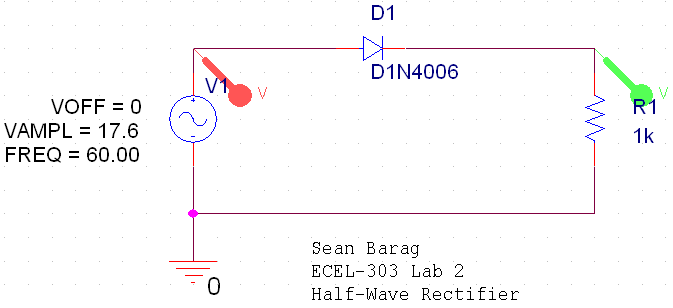
\includegraphics[width=.6\textwidth]{img/screen/halfwaveShot.PNG}
	\parbox{.6\textwidth}{
	\caption{Schematic capture of the half-wave rectifier shown initially in
		Figure~\ref{fig:schem1}.}
	\label{fig:pspice1}}
\end{figure}

\begin{figure}[H]
	\centering
	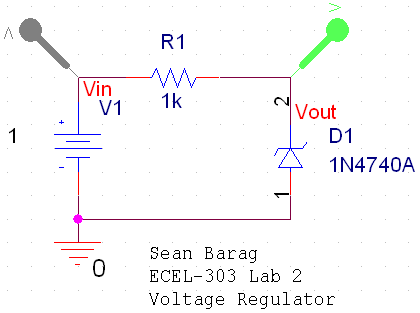
\includegraphics[width=.6\textwidth]{img/screen/voltageRegulatorShot.PNG}
	\parbox{.6\textwidth}{
	\caption{PSpice schematic for the DC voltage regulator originally drawn in
		Figure~\ref{fig:schem3}.}
	\label{fig:pspice3}}
\end{figure}

\begin{figure}[H]
	\centering
	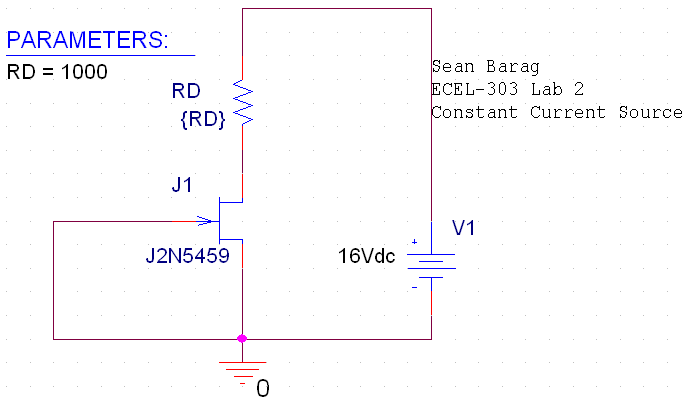
\includegraphics[width=.6\textwidth]{img/screen/constantCurrent16Shot.PNG}
	\parbox{.6\textwidth}{
	\caption{Simulated constant current source.  This circuit was originally
		presented in Figure~\ref{fig:schem4}, and has a counterpart circuit shown
		below in Figure~\ref{fig:pspice4b}.}
	\label{fig:pspice4a}}
\end{figure}

\begin{figure}[H]
	\centering
	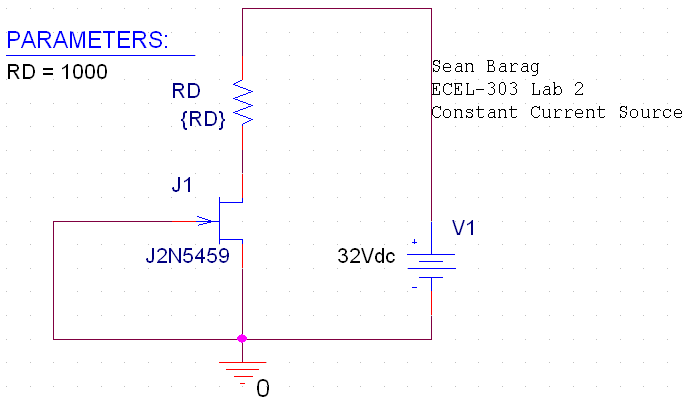
\includegraphics[width=.6\textwidth]{img/screen/constantCurrent32Shot.PNG}
	\parbox{.6\textwidth}{
	\caption{Companion circuit to the constant current source in
		Figure~\ref{fig:pspice4a}, originally drawn in Figure~\ref{fig:schem4}.
		Note the increased voltage from the DC source.}
	\label{fig:pspice4b}}
\end{figure}

\begin{figure}[H]
	\centering
	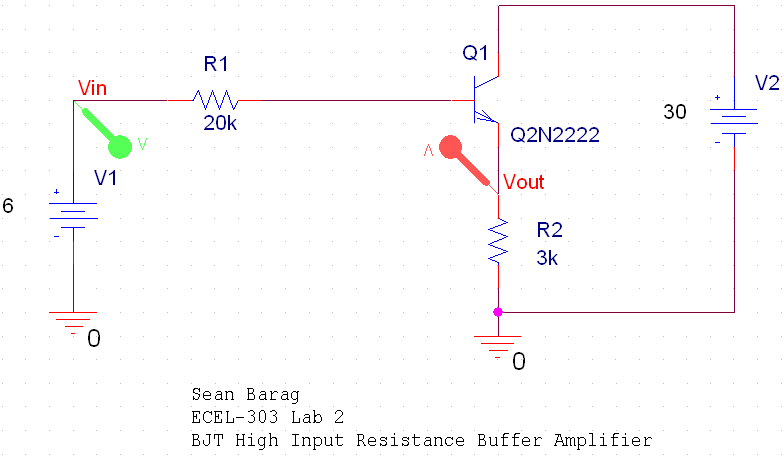
\includegraphics[width=.6\textwidth]{img/screen/bjtShot.PNG}
	\parbox{.6\textwidth}{
	\caption{Captured schematic of the BJT-based high input resistance buffer
		amplifier.  It was drawn initially in Figure~\ref{fig:schem5}.}
	\label{fig:pspice5}}
\end{figure}


\section{License}
Copyright \copyright\ 2011, Sean Barag.  All rights reserved.

Redistribution and use in source and binary forms, with or without
modification, are permitted provided that the following conditions are met:
\begin{itemize}
\item Redistributions of source code must retain the above copyright notice, this
  list of conditions and the following disclaimer.
\item Redistributions in binary form must reproduce the above copyright notice, this
  list of conditions and the following disclaimer in the documentation and/or
  other materials provided with the distribution.
\item Neither the name of the owner nor the names of its contributors may be
  used to endorse or promote products derived from this software without specific
  prior written permission.
\end{itemize}

THIS SOFTWARE IS PROVIDED BY THE COPYRIGHT HOLDERS AND CONTRIBUTORS ``AS IS'' AND
ANY EXPRESS OR IMPLIED WARRANTIES, INCLUDING, BUT NOT LIMITED TO, THE IMPLIED
WARRANTIES OF MERCHANTABILITY AND FITNESS FOR A PARTICULAR PURPOSE ARE
DISCLAIMED. IN NO EVENT SHALL THE COPYRIGHT HOLDER OR CONTRIBUTORS BE LIABLE
FOR ANY DIRECT, INDIRECT, INCIDENTAL, SPECIAL, EXEMPLARY, OR CONSEQUENTIAL
DAMAGES (INCLUDING, BUT NOT LIMITED TO, PROCUREMENT OF SUBSTITUTE GOODS OR
SERVICES; LOSS OF USE, DATA, OR PROFITS; OR BUSINESS INTERRUPTION) HOWEVER
CAUSED AND ON ANY THEORY OF LIABILITY, WHETHER IN CONTRACT, STRICT LIABILITY,
OR TORT (INCLUDING NEGLIGENCE OR OTHERWISE) ARISING IN ANY WAY OUT OF THE USE
OF THIS SOFTWARE, EVEN IF ADVISED OF THE POSSIBILITY OF SUCH DAMAGE.\\

Source code for this document is available at \texttt{http://github.com/sjbarag/}.


\end{document}
